\documentclass{xjtureport}
% =============================================
\usepackage[english]{babel} %支持混合语言
\usepackage[dvipsnames]{xcolor}
\usepackage{graphicx} 
\usepackage{amsmath} %更多数学符号
\usepackage{amssymb} %罗马字体
\usepackage{wasysym}
\usepackage[colorlinks,%提供有颜色的跳转链接
            linkcolor=blue,
            anchorcolor=blue,
            citecolor=blue,
            urlcolor=blue
            ]{hyperref}
% Renaming floats with babel
\addto\captionsenglish{
    \renewcommand{\contentsname}{目录}
    \renewcommand{\listfigurename}{插图目录}
    \renewcommand{\listtablename}{表格}
    %\renewcommand{\refname}{\sihao 参考文献}
    \renewcommand{\refname}{\sihao  \leftline{\textcolor{blue}{参考文献}}} %这几个字默认字号稍大,改成四号字,楷书,居左(默认居中) 根据喜好自行修改,官方模板未作要求
    \renewcommand{\abstractname}{摘要}
    \renewcommand{\indexname}{索引}
    \renewcommand{\tablename}{ 表}
    \renewcommand{\figurename}{图}
    } %把Figure改成‘图’,reference改成‘参考文献’。如此处理是为了避免和babel包冲突。
%定义字号
% =============================================
\major{电气工程}
\name{张三}
\title{硕士研究生实验报告}
\stuid{S130920033}
\college{自动化(人工智能)学院}
\date{\zhtoday}
\lab{寝室}
\course{开关变换器数字控制技术}
\instructor{杭丽君}
\grades{59}
\expname{Buck变换器数字峰值电流控制}
\exptype{设计实验}
\partner{李四}

\begin{document}
% =============================================
% Part 1 Header
% =============================================
\makecover
\makeheader
% =============================================
% Part 2 Main document
% =============================================
\section{实验目的}
加深对数字峰值电流Buck变换器次谐波震荡和DSC控制的了解。
\section{实验内容}
\subsection{实验参数}

为了验证DSC技术能消除单缘调制DPC中产生的次谐波震荡的理论分析,以Buck变换器为例,选择如下电路参数进行实验研究:$v_g=5 \;{\rm V}$,$L=20\;\mu{\rm H}$,$C=1420\;\mu{\rm F}$,$R_e=30\;m \Omega {\rm(ESR)}$,$T_s=20\;\mu{\rm s}$,$K_c=1$。
前缘、后缘调制和三角后缘调制,$D>0.5$,$v_o=3.3\;{\rm V}\sim4\;{\rm V}$,$R=0.3\;\Omega$

仿真平台中把数字处理器时钟频率设置为50 MHz,从0开始计数加,到999达到开关周期$20\;\mu{\rm s}$;\\DPWM的有效分辨率为10位,ADC的有效分辨率为8位。
\subsection{仿真内容}
\begin{enumerate}
    \item 仿真静态过程中的上述工作情况的三种调制方式。
    \label{仿真内容1}
    \item 具有次谐波震荡的电路采用DTC补偿后的稳态工作情况。
     \label{仿真内容2}
    \item 1.2 ms的时候,输出负载从50\%到100\%的动态过程,分别在后缘和前缘调制方式下的动态过程进行对比。
     \label{仿真内容3}
    \item 2.4 ms的时候,输出负载从100\%到30\%的动态过程,分别在后缘和前缘调制方式下的动态过程进行对比。
     \label{仿真内容4}
\end{enumerate}

\subsection{提交部分}
\begin{enumerate}
    \item 电路和调制波形图;
    \item 仿真模型和代码;
    \item 文字报告(包括波形和控制方法的解释和文字描述)。需要给出对应PWM波形、电感电流波形和输出电压波形,以及补偿后相应的三角补偿波形。
\end{enumerate}

\section{主要仪器设备}
计算机,Matlab 软件
%以下部分学生作答---------------------------------------------------
%以下部分学生作答---------------------------------------------------
%以下部分学生作答---------------------------------------------------
\section{操作方法和实验步骤}
\subsection{传输函数}
对差分方程进行处理,求出传输函数表达式。
\subsection{零极点分布图}
在此基础上,使用 Matlab 中的 \texttt{zplane} 函数进一步画出在不同 $a$ 取值情况下的零极点分布图。
\subsection{幅频响应}
之后使用 \texttt{freqz} 函数画出不同a取值情况下的频率响应图像。

\section{实验数据记录和处理}
\subsection{传输函数}
根据差分方程,传输函数如下:
$$H(z) = \frac{Y(z)}{X(z)} = \frac{z^2}{z^2-(0.5+a)z+0.5a}$$
\subsection{零极点分布图}
$a = 0.8, 0.9, 1.1$时,系统的零极点分布图及程序如下:
\begin{enumerate}
    \item 图像如图~\ref{fig:dist} 所示。
          \begin{figure}[!htbp]
              \centering
              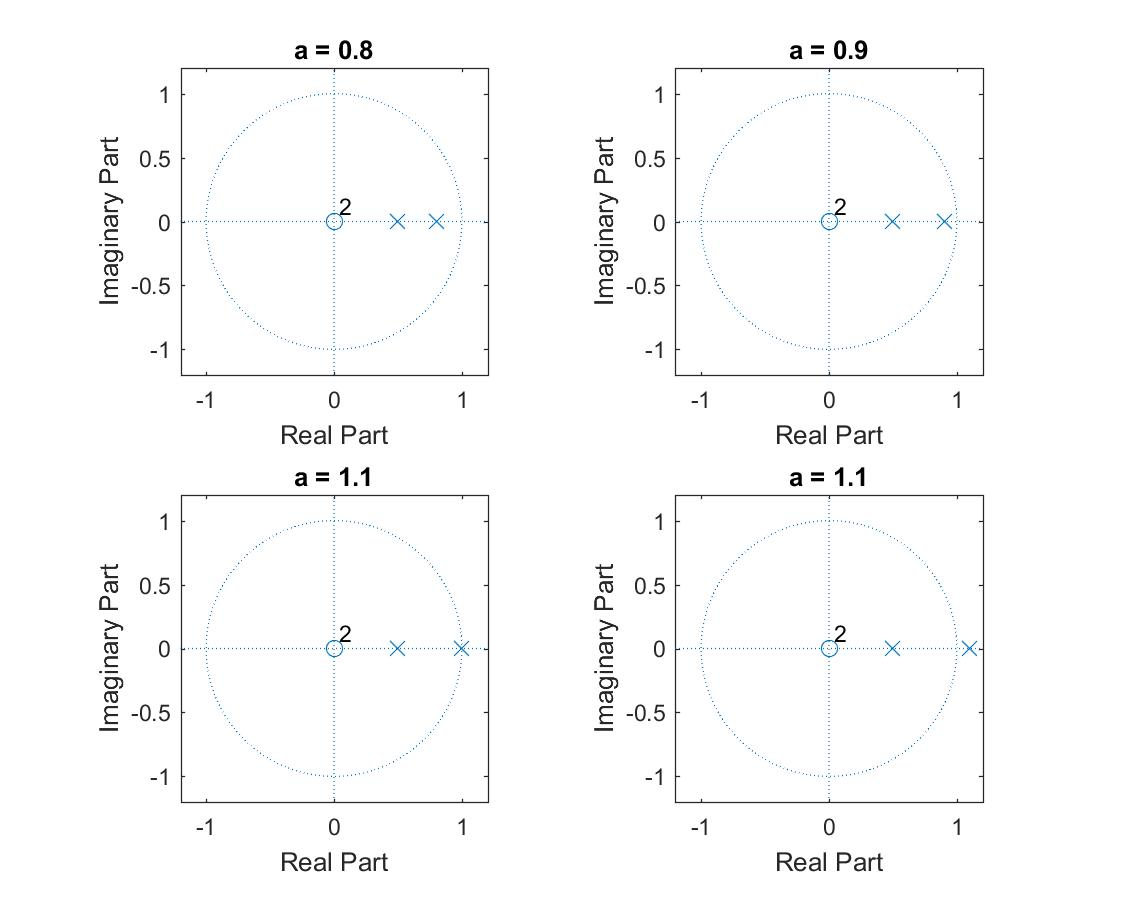
\includegraphics[width=0.6\linewidth]{01.jpg}
              \caption{系统的零极点分布图}
              \label{fig:dist}
          \end{figure}
    \item 代码
          \lstinputlisting[language=MATLAB]{code/do.m}
\end{enumerate}

\subsection{频率响应}
$a = 0.8, 0.9, 1.0, 1.1$时,系统的频率响应函数图形及程序如下:
\begin{enumerate}
    \item 图像如图~\ref{fig:resp} 所示。
          \begin{figure}[!htbp]
              \centering
              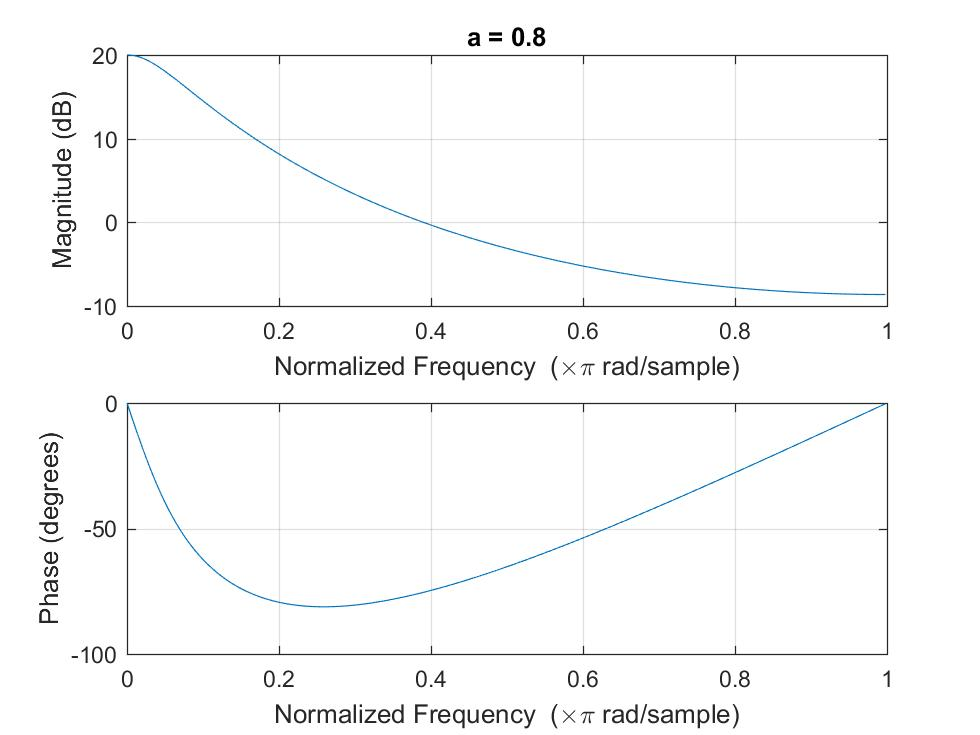
\includegraphics[width=0.6\linewidth]{02-1.jpg}
              \caption{系统的频率响应函数图形}
              \label{fig:resp}
          \end{figure}
    \item 代码
          \lstinputlisting[language=MATLAB]{code/next.m}
\end{enumerate}

\section{实验结果与分析}

Lorem ipsum dolor sit amet, consectetur adipiscing elit. Cras sit amet pharetra orci. Pellentesque ex est, ultricies non viverra sed, iaculis sed est. Suspendisse ex felis, aliquam et nulla in, vehicula gravida velit. In porttitor volutpat tincidunt. Aenean eleifend non augue sit amet ultrices. Proin rutrum odio vitae est luctus, eu facilisis leo dapibus. Aliquam commodo efficitur erat, sit amet pulvinar nulla ultrices ac. Vestibulum ullamcorper malesuada odio. Suspendisse id sollicitudin arcu. Nam fringilla commodo neque quis posuere. Sed lobortis justo nisl, ut molestie sapien semper ac. Proin in massa vel neque tempus porta id accumsan magna. Aliquam pharetra lacus ac arcu accumsan varius. Praesent condimentum mi vitae purus elementum imperdiet.

Etiam in bibendum arcu. Etiam porta metus ligula. Cras tempor, leo vel faucibus consequat, diam justo malesuada ex, et pretium risus est sit amet lectus. In sit amet efficitur quam. Maecenas quis molestie odio, et consectetur augue. Mauris erat erat, tristique a nunc in, molestie molestie lectus. Nullam commodo ornare urna, vel tincidunt libero aliquam ut. Ut hendrerit nunc id sapien tristique mollis. Aenean maximus, neque molestie dignissim cursus, augue neque dictum purus, vitae varius diam ex vitae est. Nulla bibendum facilisis semper. Nulla placerat ultricies lorem, quis consequat metus pulvinar eu. Morbi sed massa arcu. Nulla sagittis felis a suscipit elementum.

\begin{table}[!htbp]
    \begin{center}
        \begin{tabular}{lllllllll}
            \toprule
            时间 & 双蒸水-1 & 双蒸水-2 & 双蒸水-3 & 待测样本-1 & 待测样本-2 & 待测样本-3 & 双蒸水 & 待测样本  \\
            \midrule
            20s  & 0.1628 & 0.1666 & 0.1617 & 1.3338 & 1.3826 & 1.3744 & 0.1637 & 1.3636  \\
            80s  & 0.1630 & 0.1669 & 0.1619 & 1.3626 & 1.4130 & 1.4054 & 0.1639 & 1.3936 \\
            $\Delta A$  &  &  &  &  &  &  & 0.0002 & 0.0300 \\
            \bottomrule
        \end{tabular}
    \end{center}
    \caption{吸光度数据}
    \label{fig:dist}
\end{table}

\end{document}
